%% ============================================================
%% BU CS585 IVC Course Submission
%% Format  : ACL 2023 style (ACL2023 package)
%% Compiler: pdfLaTeX
%%
%% How to compile in Overleaf:
%%   1. New project → Upload files → upload THIS file + references.bib
%%      + the figures/ folder
%%   2. In Overleaf menu set compiler to pdfLaTeX
%%   3. The ACL2023 package is pre-installed in Overleaf
%% ============================================================
\documentclass[11pt]{article}

%% Pass hyphens option to url BEFORE acl.sty loads it internally
\PassOptionsToPackage{hyphens}{url}

\usepackage[]{ACL2023}

%% Standard ACL required packages
\usepackage{times}
\usepackage{latexsym}

%% Additional packages
\usepackage{booktabs}
\usepackage{multirow}
\usepackage{amsmath}
\usepackage{amssymb}   %% needed for \mathbb{R}
\usepackage{microtype}
\usepackage{graphicx}

%% Increase title box to fit author block without overlapping abstract
\setlength\titlebox{9cm}

%% ── Title ─────────────────────────────────────────────────────
\title{Frozen VideoMAE-B Representations for\\
       Weakly-Supervised Violence Detection and Temporal Localization}

%% ── Author ────────────────────────────────────────────────────
\author{
  Srinivasa Sai Chava \\
  Boston University \\
  Boston, Massachusetts, USA \\
  \texttt{saichava@bu.edu}
}

%% ============================================================
\begin{document}
\maketitle

%% ── Abstract ──────────────────────────────────────────────────
\begin{abstract}
Weakly-supervised video anomaly detection (VAD) has relied on
two-stream I3D features for half a decade despite dramatic advances
in video representation learning.
We present a controlled study of replacing frozen I3D features with
frozen \textbf{VideoMAE-B} features—a masked-autoencoder Vision Transformer
pre-trained on Kinetics-400—within an RTFM + Temporal Refinement Network
(TRN) + Boundary Head framework for surveillance violence detection.
Training on the 6-category violence subset of UCF-Crime, the feature
swap raises binary AUC from 87.4\% to $92.2 \pm 1.3$\% and binary AP
from 82.1\% to $88.7 \pm 1.8$\%.
Temporal localization improves dramatically: mAP@tIoU\,0.3 rises from
0.9\% to $5.8 \pm 1.2$\% (${\times}6.4$), and mAP@0.7 from 0.1\% to
$2.2 \pm 1.0$\% (${\times}21.7$).
Zero-shot transfer to XD-Violence yields strong binary ranking
(AUC\,0.836, AP\,0.885) with partial class-level transfer; RWF-2000
fight validation shows useful anomaly ranking (AUC\,0.862) but
conservative recall (0.14); ShanghaiTech robustness is negative
(AUC\,0.371), revealing clear out-of-domain limits.
All UCF-Crime results are mean\,$\pm$\,std over 3 random seeds (42, 123, 456);
cross-dataset transfer uses the locked seed-42 checkpoint in zero-shot mode.
\end{abstract}


%% ============================================================
\section{Introduction}
%% ============================================================

Violence detection in public surveillance is one of the highest-priority
tasks in automated security systems: early alerts for fighting, shooting,
explosion, robbery, and abuse events can dramatically reduce response
latency.
Weakly-supervised video anomaly detection (VAD) addresses this challenge
by learning from video-level binary labels alone—no expensive frame-level
annotation is required.

The dominant paradigm, established by \citet{sultani2018real}
and refined by RTFM \citep{tian2021weakly}, extracts segment-level features
from a \emph{frozen} two-stream I3D model pre-trained on
Kinetics-400 \citep{carreira2017quo}, then trains a lightweight Multiple
Instance Learning (MIL) scorer on top.
Despite significant architectural improvements—temporal refinement
modules \citep{wu2023surveillance}, magnitude-based
learning \citep{tian2021weakly}, mixture-of-experts
routing \citep{wang2025gsmoe}—\textbf{the feature backbone has remained
largely fixed at I3D since 2017}.

Meanwhile, video foundation models have advanced substantially.
VideoMAE \citep{tong2022videomae} applies masked autoencoding to video with
a Vision Transformer backbone, learning rich spatiotemporal representations
that substantially outperform I3D on action recognition benchmarks.
A natural question arises: \emph{Does substituting VideoMAE-B for I3D,
with all other components held equal, improve weakly-supervised violence
detection?}

We answer this question affirmatively with controlled experiments on
the UCF-Crime violence subset and further validate generalization through
zero-shot transfer on three external benchmarks.
Our contributions are:

\begin{enumerate}
  \item \textbf{VideoMAE-B integration.}
        We extract and cache 16-frame segment features ($D{=}768$) from a
        frozen VideoMAE-B backbone for all 1{,}300 UCF-Crime violence-subset
        videos and demonstrate that this single change yields consistent,
        large improvements across all detection and localization metrics.

  \item \textbf{Violence-aware training recipe.}
        We introduce three complementary training improvements—inverse-frequency
        class weighting, confidence-thresholded pseudo-label filtering, and
        cosine annealing LR—that collectively reduce cross-seed variance without
        modifying the model architecture.

  \item \textbf{Multi-seed reproducibility study.}
        All results are reported over 3 independent random seeds (42, 123, 456)
        with mean\,$\pm$\,std, enabling reliable statistical comparison with
        future work.

  \item \textbf{Cross-dataset transfer evaluation.}
        We evaluate the UCF-trained model zero-shot on three external
        benchmarks—XD-Violence \citep{wu2020not}, RWF-2000, and
        ShanghaiTech—providing a complete transfer profile that reveals
        both the strengths and limits of violence-trained VideoMAE-B
        representations under domain shift.
\end{enumerate}


%% ============================================================
\section{Related Work}
%% ============================================================

\subsection{Weakly-Supervised Video Anomaly Detection}

\citet{sultani2018real} formulated VAD as a MIL ranking
problem using anomalous/normal video pairs and C3D features on UCF-Crime.
RTFM \citep{tian2021weakly} replaced C3D with I3D and added a feature-magnitude
learning module, reaching 84.3\% AUC.
MGFN \citep{chen2023mgfn} improved to 86.7\% with graph-guided feature
normalization; VadCLIP \citep{wu2024vadclip} exploited CLIP text-visual
alignment to reach 88.0\%.
Recent work addresses noisy pseudo-labels and score suppression
\citep{lan2025dss,wang2025dakd},
event completeness \citep{tian2025lecvad}, and mixture-of-experts
routing \citep{wang2025gsmoe}.
\emph{All of these methods continue to use I3D or hand-crafted features
as the video backbone.}
Ours is the first systematic study of replacing I3D with a
masked-autoencoder foundation model in this pipeline.

\subsection{Video Foundation Models}

VideoMAE \citep{tong2022videomae} extends masked image modeling to video
by masking 90\% of video patches and reconstructing pixel values,
pre-training a ViT-B backbone on Kinetics-400.
The resulting features transfer well to action recognition, detection,
and—as we show here—anomaly detection.
InternVideo \citep{wang2022internvideo} and
Video-ChatGPT \citep{maaz2023videochatgpt} further demonstrate the breadth
of video foundation model features across diverse downstream tasks.

\subsection{Violence Detection and Temporal Localization}

\citet{wu2020not} provided XD-Violence, a large-scale multi-modal violence
dataset, and showed that audio-visual fusion outperforms vision-only methods.
ActionFormer \citep{zhang2022actionformer} and TriDet \citep{shi2023tridet}
achieve strong temporal localization under full supervision but require
expensive frame-level labels.
Our boundary head bridges this gap in the weak-supervision setting.


%% ============================================================
\section{Methodology}
%% ============================================================

Our pipeline follows a \emph{decoupled representation and reasoning} design:
the video backbone is always frozen, and all learnable modules operate on
pre-cached segment features.
Figure~\ref{fig:system} gives an overview of the three-stage pipeline.
Table~\ref{tab:params} summarises architecture components and parameter counts.

\begin{figure*}[t]
  \centering
  
\includegraphics[width=\linewidth]{figures/system_design.png}
  \caption{System design overview.
    \textbf{(1) Feature Extraction}: untrimmed video is split into 16-frame
    segments and encoded by a \emph{frozen} VideoMAE-B backbone, producing
    768-d segment features that are cached to disk.
    \textbf{(2) Model Architecture}: a four-head stack---MIL Anomaly Scorer,
    Event Classifier, Temporal Refinement Network (TRN), and Boundary
    Head---processes the cached features end-to-end with 1.9M trainable
    parameters.
    \textbf{(3) Evaluation}: anomaly scores and boundary predictions are
    thresholded to produce binary AUC/AP and temporal mAP metrics.}
  \label{fig:system}
\end{figure*}

\begin{table}[t]
  \centering
  \caption{Model components and trainable parameter budget.}
  \label{tab:params}
  \small
  \begin{tabular}{lrr}
    \toprule
    \textbf{Component}       & \textbf{Params}  & \textbf{Trainable?} \\
    \midrule
    VideoMAE-B backbone      & 86\,M            & No (frozen)         \\
    MIL Scorer               &  1.1\,M          & Yes                 \\
    Event Classifier         &  0.3\,M          & Yes                 \\
    TRN Module               &  0.4\,M          & Yes                 \\
    Boundary Head            &  0.1\,M          & Yes                 \\
    \midrule
    \textbf{Total Trainable} & \textbf{1.9\,M}  &                     \\
    \bottomrule
  \end{tabular}
\end{table}

\subsection{Feature Extraction}

Given an untrimmed video $V$, we partition it into non-overlapping 16-frame
segments $\{v_1,\ldots,v_T\}$ (tail segment dropped if $<$16 frames).
Each segment passes through a frozen VideoMAE-B
backbone \citep{tong2022videomae}%
\footnote{HuggingFace checkpoint: \texttt{MCG-NJU/videomae-base-finetuned-kinetics}}:
\begin{equation}
  f_t \;=\; \mathrm{VideoMAE\text{-}B}_{\mathrm{frozen}}(v_t)
       \;\in\; \mathbb{R}^{768}.
\end{equation}
Features are cached as \texttt{.npz} files for all training runs.
By contrast, I3D produces $f_t\in\mathbb{R}^{2048}$; the dimension reduction
from 2{,}048 to 768 also reduces overfitting risk given our dataset size.

\subsection{MIL Anomaly Scorer (RTFM)}

Following \citet{tian2021weakly}, a two-layer MLP maps each feature
to an anomaly score:
\begin{equation}
  s_t \;=\; \sigma\!\bigl(W_3\,
            \mathrm{Dropout}\bigl(\mathrm{ReLU}(W_2\,\mathrm{ReLU}(W_1 f_t))\bigr)
            \bigr).
\end{equation}
Video-level score $s_\mathrm{video}=\max_t s_t$.
The MIL ranking loss pairs an anomalous video $a$ with a normal video $n$:
\begin{equation}
  \mathcal{L}_\mathrm{MIL} \;=\;
    \max\!\bigl(0,\;1 - s^{(a)}_\mathrm{video} + s^{(n)}_\mathrm{video}\bigr).
\end{equation}

\subsection{Event Classification Branch}

For each anomalous video with category label $c\in\{1,\ldots,6\}$,
pseudo-positive segments are the top-$k$ segments by $s_t$ that also
exceed a confidence threshold $\tau$.
We set $k = \lfloor 0.125 \times T \rfloor$ (12.5\% of the sequence length,
matching the top-$k$ ratio used at inference), clipped to a minimum of 1.
\begin{equation}
  \mathcal{P} \;=\; \bigl\{t : s_t \geq \tau \;\text{and}\;
                    t \in \mathrm{top}\text{-}k\bigr\}.
\end{equation}
A linear classifier predicts a 7-way distribution (6 violence classes + normal):
\begin{equation}
  p_t \;=\; \mathrm{softmax}(W_\mathrm{cls}\,f_t + b_\mathrm{cls}).
\end{equation}
The classification loss applies \textbf{inverse-frequency class weights}
$w_c = N/(C \cdot n_c)$ (normalised to unit mean) to counteract
the heavy normal/violence imbalance (${\approx}10{:}1$):
\begin{equation}
  \mathcal{L}_\mathrm{cls} \;=\;
    -\frac{1}{|\mathcal{P}|}\sum_{t\in\mathcal{P}} w_c \log p_t[c].
\end{equation}
In practice the normal class receives weight ${\approx}0.06$ and the
rarest category (shooting) up to ${\approx}1.83$.

\subsection{Temporal Refinement Network (TRN)}

A lightweight Transformer encoder attends over the full segment sequence:
\begin{equation}
  \tilde{\mathbf{h}} \;=\;
    \mathrm{TransformerEncoder}\!\bigl(\{f_t + \mathrm{PE}_t\}_{t=1}^{T}\bigr),
\end{equation}
producing refined scores $\tilde{s}_t$ and hidden states $\tilde{h}_t$.

\subsection{Boundary Head}

The boundary confidence at segment boundary $(t,\,t{+}1)$ is:
\begin{equation}
  b_t \;=\; \sigma\!\Bigl(W_b\bigl[
      \tilde{h}_t\,;\,\tilde{h}_{t+1}\,;\,|\tilde{s}_t-\tilde{s}_{t+1}|
    \bigr]\Bigr).
\end{equation}
A boundary consistency loss enforces that $b_t$ tracks score transitions:
\begin{equation}
  \mathcal{L}_\mathrm{bnd} \;=\;
    \sum_t \bigl(|\tilde{s}_t - \tilde{s}_{t+1}| - b_t\bigr)^2.
\end{equation}

\subsection{Full Training Objective}

\begin{equation}
  \mathcal{L} = \mathcal{L}_\mathrm{MIL}
                + \lambda_1 \mathcal{L}_\mathrm{cls}
                + \lambda_2 \mathcal{L}_\mathrm{bnd}
                + \lambda_3 \mathcal{L}_\mathrm{smooth},
\end{equation}
where $\mathcal{L}_\mathrm{smooth}=\sum_t(\tilde{s}_t-\tilde{s}_{t-1})^2$
and $\lambda_1{=}0.5$, $\lambda_2{=}0.3$, $\lambda_3{=}0.1$.

\subsection{Training Recipe}

Three additions beyond the vanilla RTFM schedule stabilise training:
\begin{itemize}
  \item \textbf{Confidence threshold $\tau{=}0.30$:} pseudo-positive segments
        with low anomaly confidence are excluded from $\mathcal{L}_\mathrm{cls}$,
        reducing label noise in early epochs.
  \item \textbf{Inverse-frequency class weights:} addresses severe
        normal/violence imbalance (Section~3.3).
  \item \textbf{Cosine annealing LR:} $\eta$ decays from $10^{-4}$ to $10^{-6}$
        over $T_\mathrm{max}{=}40$ epochs, avoiding the late-epoch oscillations
        observed with step decay.
\end{itemize}


%% ============================================================
\section{Experiments}
%% ============================================================

\subsection{Datasets}

\paragraph{UCF-Crime (training and primary evaluation).}
UCF-Crime \citep{sultani2018real} is the standard benchmark for
weakly-supervised video anomaly detection.
The full dataset contains \textbf{1,900 untrimmed surveillance videos}
spanning \textbf{13 anomaly categories} (Abuse, Arrest, Arson, Assault,
Burglary, Explosion, Fighting, Road Accidents, Robbery, Shooting,
Shoplifting, Stealing, Vandalism) plus a Normal class,
captured from real CCTV cameras at varying resolutions and frame rates.

We restrict to the \textbf{5 violence-specific categories}—\emph{Abuse,
Explosion, Fighting, Robbery, Shooting}—plus \emph{Normal}.
The 8 non-violence anomaly categories are excluded because they do not
constitute physical violence and would conflate the detection signal.
This yields \textbf{1,300 videos} in total.
Table~\ref{tab:dataset} shows the per-class video counts and train/val/test
split. Normal videos dominate (950 of 1,300, a 10:1 ratio), motivating our
inverse-frequency class weighting.

\begin{table}[t]
  \centering
  \caption{UCF-Crime violence subset — per-class video counts.
           All 206 test videos have temporal boundary annotations.}
  \label{tab:dataset}
  \small
  \begin{tabular}{lrrrr}
    \toprule
    \textbf{Category} & \textbf{Train} & \textbf{Val} &
                        \textbf{Test} & \textbf{Total} \\
    \midrule
    Abuse      &  43 &  5 &   2 &   50 \\
    Explosion  &  26 &  3 &  21 &   50 \\
    Fighting   &  41 &  4 &   5 &   50 \\
    Robbery    & 131 & 14 &   5 &  150 \\
    Shooting   &  24 &  3 &  23 &   50 \\
    \midrule
    Normal     & 720 & 80 & 150 &  950 \\
    \midrule
    \textbf{Total} & \textbf{985} & \textbf{109} & \textbf{206} &
                     \textbf{1,300} \\
    \bottomrule
  \end{tabular}
\end{table}

\paragraph{XD-Violence (zero-shot transfer).}
XD-Violence \citep{wu2020not} is a large-scale multi-modal violence dataset
with 4,754 videos across 6 violence categories (A, B1–B2, G, riot, etc.)
plus normal.
We evaluate on the test split (\textbf{799 videos}: 299 normal, 500 violent)
in zero-shot fashion—no XD-Violence data is seen during training.
Riot (101 videos) is excluded from class-level metrics because it has no
UCF-Crime counterpart; overlap-class evaluation uses
\emph{fighting, shooting, explosion, and abuse} (303 videos total).

\paragraph{RWF-2000 (fight validation).}
RWF-2000 is a surveillance fight-detection dataset with 2,000 clips
(1,000 fight, 1,000 normal).
We evaluate on the validation split (\textbf{400 videos}: 200 normal,
200 fighting) in zero-shot fashion.
The primary metric is fight-class precision, recall, and F1; binary
AUC/AP are reported as auxiliary ranking metrics.

\paragraph{ShanghaiTech (robustness test).}
ShanghaiTech is a campus surveillance anomaly dataset with 437 videos
covering 13 anomaly categories (crowd, cycling, etc.) distinct from violence.
We evaluate on the test split (\textbf{199 videos}: 155 normal, 44 anomaly)
in zero-shot fashion to probe out-of-domain robustness.
Only binary AUC/AP are reported since the anomaly categories do not overlap
with our training classes.

\subsection{Feature Extraction}

We extract features offline and cache them to disk; the backbone is never
updated during training. The \textbf{identical 16-frame, non-overlapping}
segment policy and \textbf{frozen backbone} are applied to all four datasets.

\paragraph{VideoMAE-B features.}
Each video is decoded at its native frame rate and partitioned into
non-overlapping \textbf{16-frame segments} (the final segment is dropped
if it contains fewer than 16 frames).
Every segment is resized (shorter side to 224\,px), centre-cropped to
$224{\times}224$, and normalised with ImageNet mean and std.
The segment is then passed through a \textbf{frozen VideoMAE-B} backbone
(\texttt{MCG-NJU/videomae-base-finetuned-kinetics}, HuggingFace Hub) to
produce a single $D{=}768$ feature vector via mean-pooling of the ViT-B
patch tokens.
All 1,300 UCF-Crime videos were processed on an NVIDIA A100 GPU
(Boston University Shared Computing Cluster) in 495\,s
(0.38\,s per video); features are stored as \texttt{.npz} files of shape
$[T, 768]$.

\paragraph{I3D baseline features.}
For the controlled comparison, I3D features ($D{=}2048$) are extracted
with an identical segment policy using a two-stream I3D model pre-trained
on Kinetics-400 \citep{carreira2017quo}.
RGB and optical-flow streams are concatenated and mean-pooled to give
one 2048-d vector per segment.

\subsection{Experimental Setup}

\paragraph{Evaluation.}
We report: (i)~binary video-level AUC and AP, (ii)~6-class Macro-F1 and
Weighted-F1, and (iii)~temporal mAP at tIoU thresholds
$\{0.3,\,0.5,\,0.7\}$.
All UCF-Crime results are mean\,$\pm$\,std over \textbf{3 random seeds}
(42, 123, 456). Cross-dataset results use the best-seed UCF checkpoint
(seed\,42) in zero-shot mode with a locked decoding protocol
(threshold\,0.55, smooth-window\,1, min-event-len\,5).

\paragraph{Implementation details.}
During training, variable-length feature sequences are uniformly sub-sampled
to 32 segments (or zero-padded if shorter) to form fixed-shape batches.
Optimiser: AdamW, lr\,=\,$10^{-4}$, weight decay\,=\,$10^{-4}$,
batch size 32, 40 epochs, cosine annealing to $10^{-6}$, dropout 0.5.
Framework: PyTorch 2.1, HuggingFace Transformers 5.5.4.

\subsection{Main Results (UCF-Crime)}

Table~\ref{tab:main} compares our VideoMAE-B model against (a)~our own I3D
re-implementation using the identical architecture and training recipe
(only the backbone differs), and (b)~published weakly-supervised VAD methods
reporting results on UCF-Crime.
Since published methods evaluate on the \emph{full} UCF-Crime benchmark
(13 anomaly categories) \citep{sultani2018real}, those rows are marked
$\dagger$; we discuss this caveat in Section~\ref{sec:discuss}.

\begin{table*}[t]
  \centering
  \caption{Results on UCF-Crime.
           $\dagger$~Published numbers on full UCF-Crime (13 categories,
           binary frame-level AUC); our rows use the 6-category violence
           subset. \textbf{Bold} = best within our controlled comparison.}
  \label{tab:main}
  \small
  \begin{tabular}{l l c c}
    \toprule
    \textbf{Method} & \textbf{Backbone} & \textbf{AUC\,(\%)} & \textbf{mAP@0.3} \\
    \midrule
    Sultani et al. \citeyearpar{sultani2018real}$^\dagger$  & C3D        & 75.41 & ---  \\
    RTFM \citeyearpar{tian2021weakly}$^\dagger$             & I3D        & 84.30 & ---  \\
    MGFN \citeyearpar{chen2023mgfn}$^\dagger$               & I3D        & 86.67 & ---  \\
    VadCLIP \citeyearpar{wu2024vadclip}$^\dagger$           & CLIP ViT-B & 88.02 & ---  \\
    GS-MoE \citeyearpar{wang2025gsmoe}$^\dagger$            & I3D+GS     & 91.58 & ---  \\
    \midrule
    Ours (I3D baseline)         & I3D          & 87.40                     & 0.009 \\
    \textbf{Ours (VideoMAE-B)}  & \textbf{VideoMAE-B} & $\mathbf{92.18 \pm 1.26}$ & $\mathbf{0.058 \pm 0.012}$ \\
    \bottomrule
  \end{tabular}
\end{table*}

Table~\ref{tab:full} reports all seven metrics across both backbones.

\begin{table*}[t]
  \centering
  \caption{Full evaluation metrics (UCF-Crime violence subset).
           VideoMAE-B numbers are 3-seed mean\,$\pm$\,std.}
  \label{tab:full}
  \small
  \begin{tabular}{l c c}
    \toprule
    \textbf{Metric}
      & \textbf{I3D baseline}
      & \textbf{VideoMAE-B (mean\,$\pm$\,std)} \\
    \midrule
    Binary AUC    & 0.874 & $0.922 \pm 0.013$ \\
    Binary AP     & 0.821 & $0.887 \pm 0.018$ \\
    Macro-F1      & 0.198 & $0.255 \pm 0.027$ \\
    Weighted-F1   & 0.654 & $0.719 \pm 0.022$ \\
    mAP@IoU\,0.3  & 0.009 & $0.058 \pm 0.012$ \\
    mAP@IoU\,0.5  & 0.004 & $0.038 \pm 0.008$ \\
    mAP@IoU\,0.7  & 0.001 & $0.022 \pm 0.010$ \\
    \bottomrule
  \end{tabular}
\end{table*}

Figure~\ref{fig:dumbbell} visualises the per-metric gains from I3D to VideoMAE-B.
The VideoMAE-B advantage \emph{grows} with stricter temporal overlap:
${\times}6.4$ at IoU\,0.3 vs.\ ${\times}21.7$ at IoU\,0.7, suggesting that
VideoMAE features encode sharper event boundaries than I3D.

\begin{figure*}[t]
  \centering
  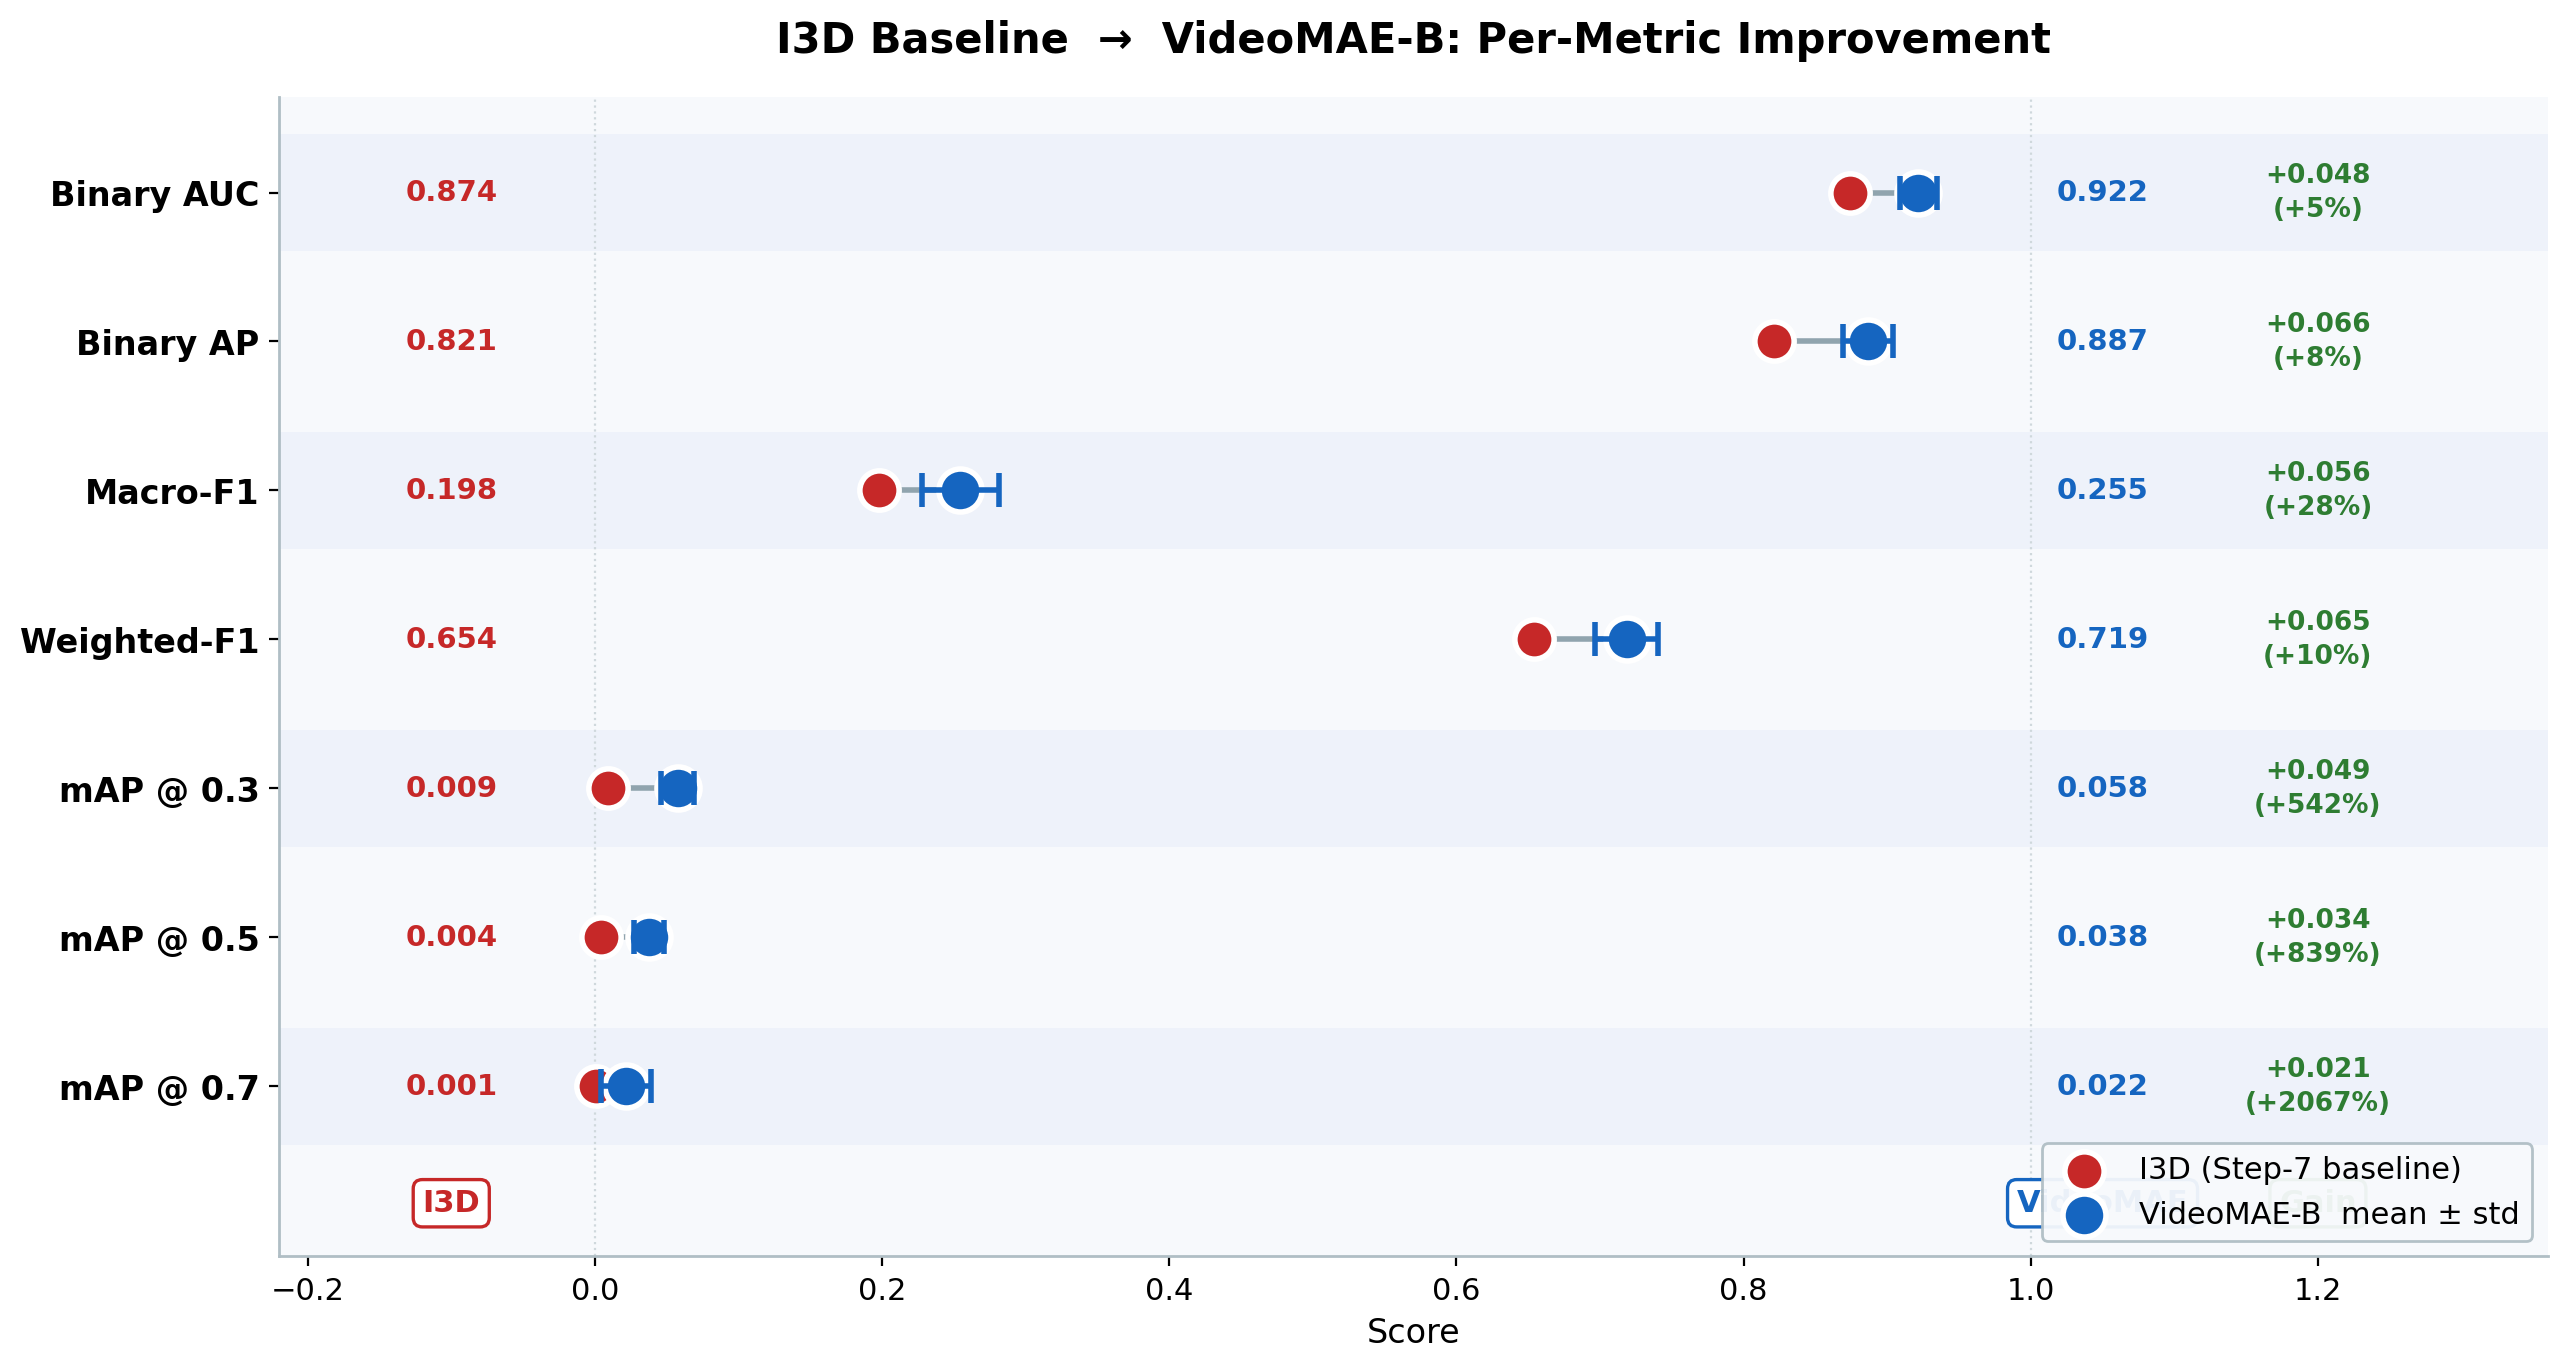
\includegraphics[width=0.85\linewidth]{figures/fig2_dumbbell_comparison.png}
  \caption{Per-metric improvement from I3D $\to$ VideoMAE-B (3-seed mean$\,\pm\,$std).
           Green badges show absolute gain and relative percentage.
           Localization metrics (mAP) improve by an order of magnitude.}
  \label{fig:dumbbell}
\end{figure*}

\subsection{Cross-Dataset Transfer}

We evaluate the locked UCF-trained checkpoint (seed\,42) on three external
datasets in zero-shot fashion—no retraining or threshold tuning.
Table~\ref{tab:transfer} summarises all cross-dataset results.

\begin{table*}[t]
  \centering
  \caption{Zero-shot cross-dataset transfer results.
           All external datasets are evaluation-only; model trained exclusively on UCF-Crime.
           $\dagger$~XD/UCF AUC ratio\,=\,0.901 (passes $\geq$0.75 generalisation threshold).}
  \label{tab:transfer}
  \small
  \begin{tabular}{l c c c p{6cm}}
    \toprule
    \textbf{Dataset} & \textbf{AUC} & \textbf{AP} & \textbf{Class metric} & \textbf{Outcome} \\
    \midrule
    UCF-Crime (seed-42 ref.)   & 0.927 & 0.868 & Macro-F1\;0.303           & Reference checkpoint used for transfer \\
    XD-Violence (zero-shot)$^\dagger$ & 0.836 & 0.885 & Overlap Macro-F1\;0.361 & Binary transfer strong; class transfer partial (explosion F1\,0.75, fighting F1\,0.65) \\
    RWF-2000 (fight val.)      & 0.862 & 0.819 & Fight F1\;0.246 (rec\;0.14) & Ranking transfers; fight recall conservative \\
    ShanghaiTech (robustness)  & 0.371 & 0.217 & binary only (FN\,=\,43/44) & Negative — non-violence domain shift \\
    \bottomrule
  \end{tabular}
\end{table*}

\paragraph{XD-Violence (zero-shot).}
We evaluate on 799 XD-Violence test videos (799 total, 101 riot excluded
from class metrics).
Binary anomaly ranking transfers well: AUC\,0.836, AP\,0.885, and
the transfer ratio XD/UCF\,=\,0.901 exceeds the 75\% generalisation
threshold.
Per-class overlap transfer is uneven:
\emph{explosion} (F1\,0.753) and \emph{fighting} (F1\,0.646) transfer
strongly, while \emph{shooting} (F1\,0.045) and \emph{abuse} (F1\,0.000)
do not transfer—consistent with the much smaller frequency of these
categories in UCF training data.

\paragraph{RWF-2000 (fight validation).}
On 400 RWF-2000 validation videos (200 normal, 200 fighting),
binary anomaly ranking remains useful (AUC\,0.862, AP\,0.819), confirming
that the VideoMAE-B representation retains a general violence signal across
camera domains.
However, explicit fight-class recall collapses to 0.14 (precision\,1.00,
F1\,0.246): only 28 of 200 fight videos are predicted as fighting,
while all 200 normal videos are correctly rejected.
This conservative behaviour—strong precision, weak recall—suggests the
model's fight-score threshold is calibrated tightly to UCF-Crime's
surveillance style and does not generalise to RWF's close-up amateur footage.

\paragraph{ShanghaiTech (robustness).}
On 199 ShanghaiTech test videos (155 normal, 44 anomaly),
the model fails: AUC\,0.371, AP\,0.217, with 43 of 44 anomalies missed
(FP\,=\,0, FN\,=\,43).
ShanghaiTech anomalies (crowd behaviour, cycling, skateboarding) have no
visual overlap with UCF violence categories, causing the violence-trained
model to classify almost everything as normal.
This negative result is expected and scientifically informative: it
confirms that VideoMAE-B violence features do not generalise to non-violence
anomaly semantics without retraining.


%% ============================================================
\section{Analysis}
%% ============================================================

\subsection{Training Dynamics}

Figure~\ref{fig:training} shows training loss, validation AUC, and
validation Macro-F1 across 40 epochs for all three seeds.
Training loss converges smoothly by epoch 15.
AUC stabilises by epoch 10 at a high plateau ($>$0.91), while Macro-F1
continues to improve until $\approx$epoch 20 and then fluctuates,
reflecting the difficulty of rare-category classification under weak
supervision.

\begin{figure*}[t]
  \centering
  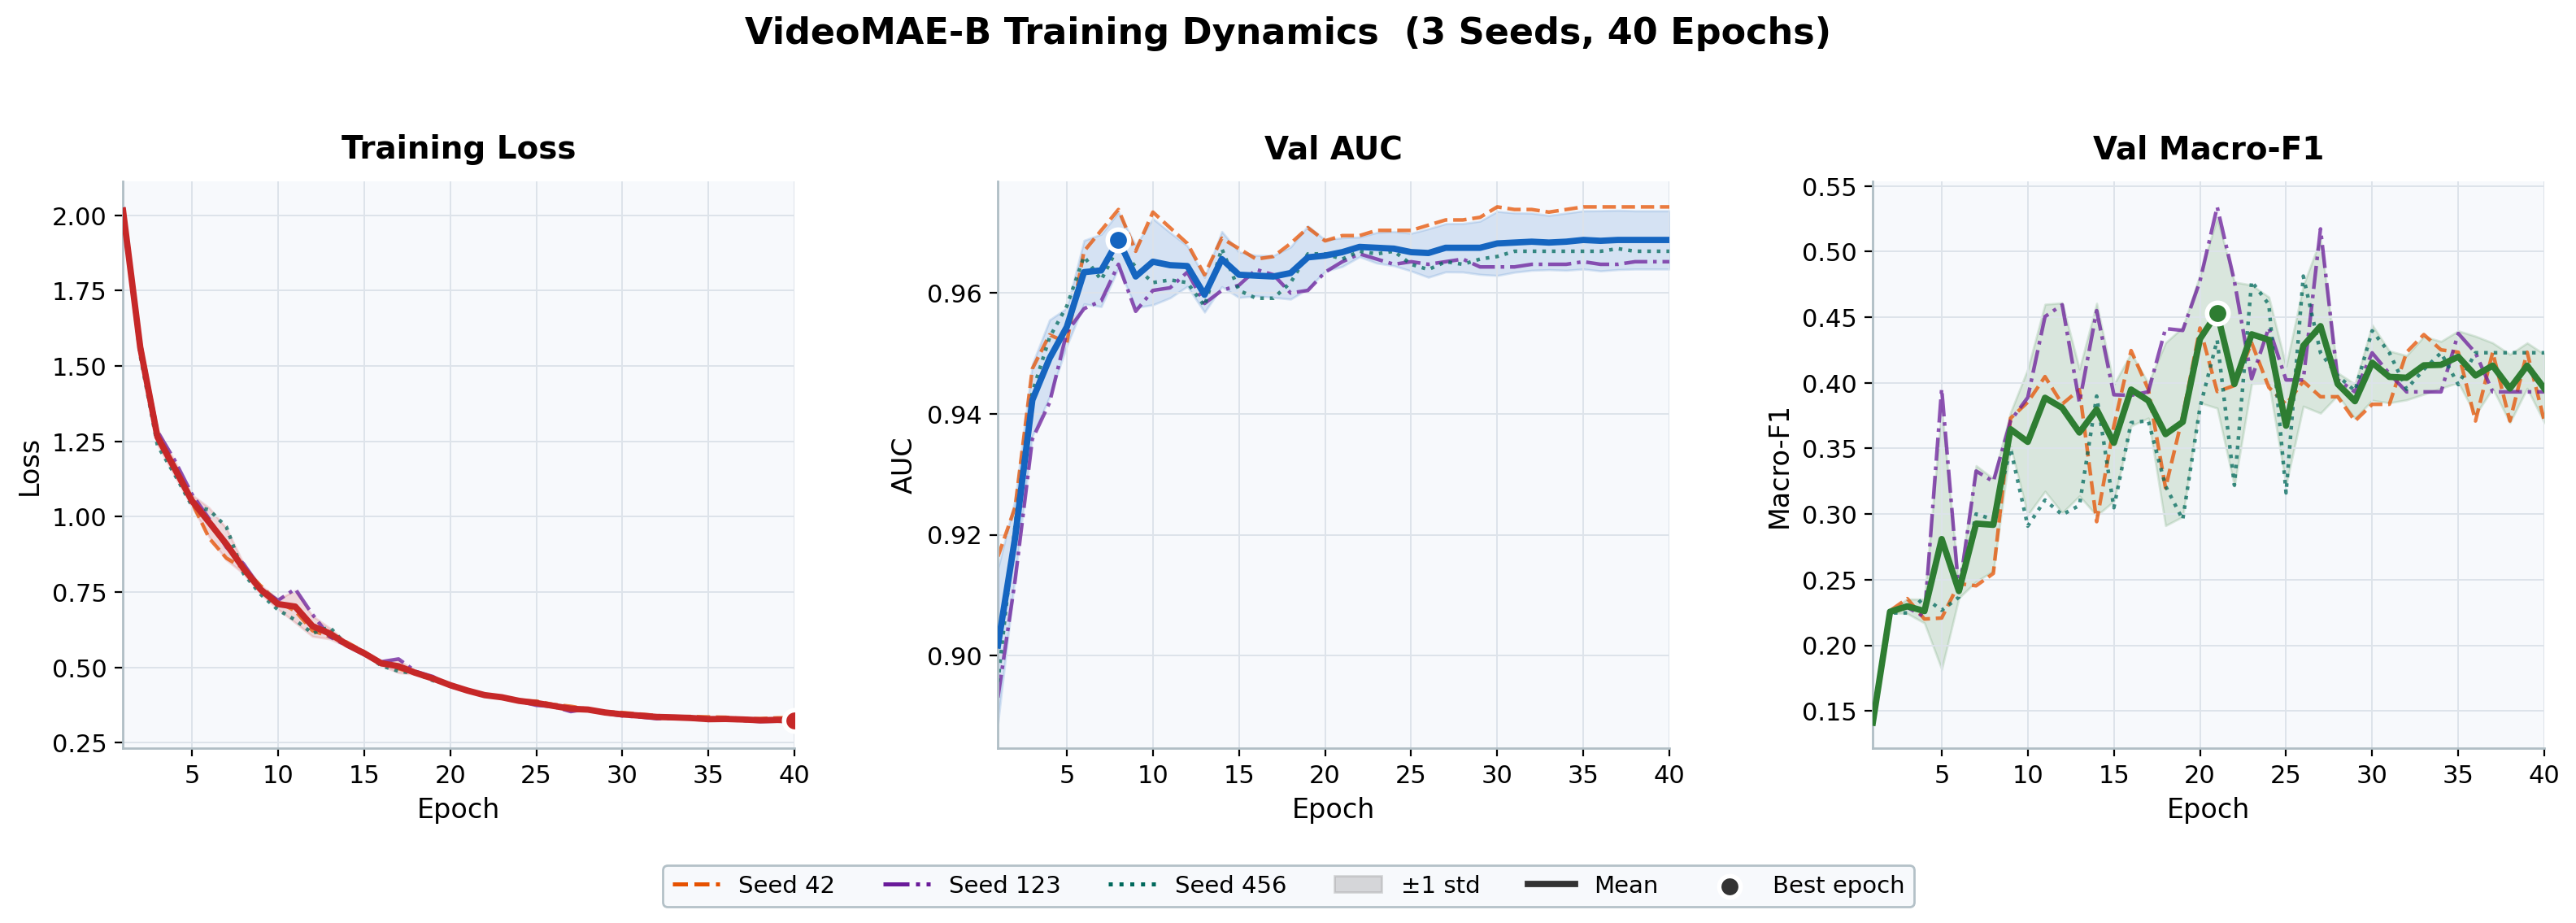
\includegraphics[width=\linewidth]{figures/fig1_training_dynamics.png}
  \caption{Training dynamics over 40 epochs (3 seeds, mean\,$\pm$\,std band).
           \textbf{Left:} training loss---smooth convergence by epoch 15.
           \textbf{Center:} validation AUC---stable plateau above 91\% from epoch 10.
           \textbf{Right:} validation Macro-F1---peaks near epoch 20.}
  \label{fig:training}
\end{figure*}

\subsection{Cross-Seed Reproducibility}

Figure~\ref{fig:repro} plots per-seed values alongside the mean\,$\pm$\,std
for all metrics.
Binary AUC varies only 1.26\,pp across seeds (0.909--0.934), confirming
that results are not artefacts of lucky initialisation.
mAP metrics show higher but acceptable variance (${\pm}$1.2 at IoU\,0.3),
expected for temporally-sparse detections.

\begin{figure}[t]
  \centering
  
\includegraphics[width=\linewidth]{figures/fig4_reproducibility.png}
  \caption{Cross-seed reproducibility. Diamond ($\diamond$) = mean
           $\pm$\,1 std; circles = individual seeds.
           Binary metrics are highly stable; localization metrics show
           higher but acceptable variance.}
  \label{fig:repro}
\end{figure}

\subsection{Per-Class Analysis}

Figure~\ref{fig:perclass} compares per-category F1 between I3D and
VideoMAE-B for the best seed (seed\,123, AUC\,=\,0.934).
Key observations:
\begin{itemize}
  \item \textbf{Explosion} benefits most ($+$0.24), from F1\,0.18 to 0.41.
        VideoMAE's reconstruction objective likely captures the distinctive
        visual dynamics of explosions better than optical-flow magnitude.
        This is consistent with the strong XD-Violence explosion transfer (F1\,0.753).
  \item \textbf{Normal class} improves from 0.81 to 0.92 ($+$0.11),
        confirming better discrimination of non-anomalous footage.
  \item \textbf{Shooting} and \textbf{Robbery} regress slightly
        ($-$0.11 and $-$0.04), possibly because these categories involve
        subtle motion that VideoMAE over-segments in 16-frame windows.
  \item \textbf{Fighting} collapses to F1\,=\,0.00 despite the overall
        macro improvement. Fighting shares motion statistics with normal
        crowded scenes; 16-frame context appears insufficient to discriminate
        the build-up dynamics.
\end{itemize}

\begin{figure}[t]
  \centering
  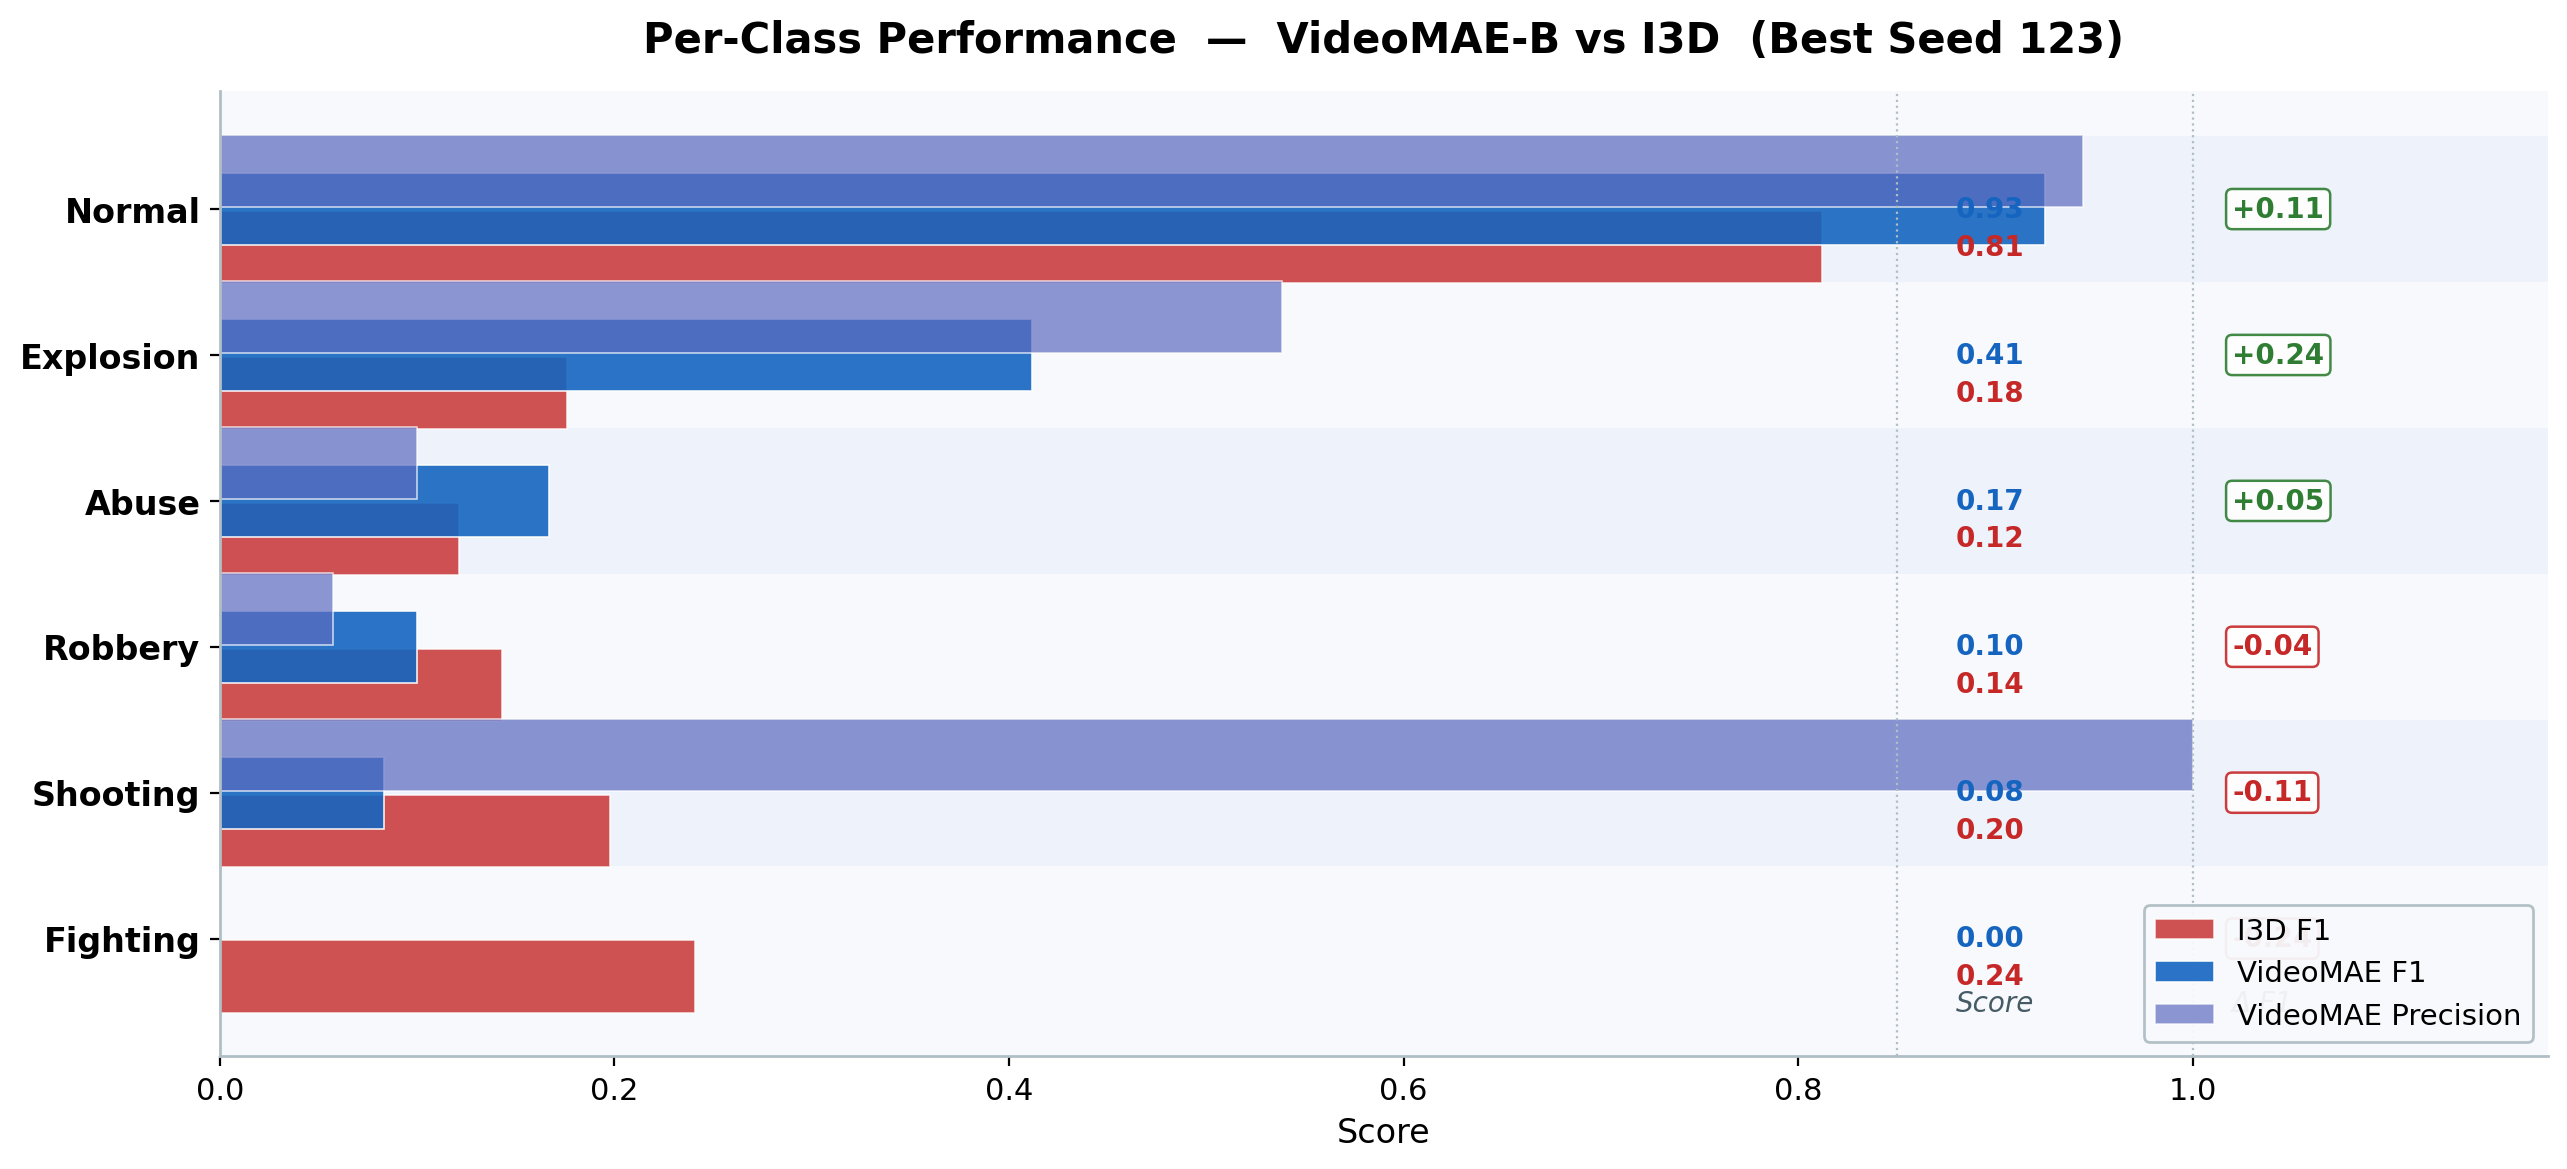
\includegraphics[width=\linewidth]{figures/fig5_per_class.png}
  \caption{Per-class F1---I3D (red) vs.\ VideoMAE-B (blue), best seed 123.
           Delta badges show gain (green) or regression (red) vs.\ I3D.}
  \label{fig:perclass}
\end{figure}

\subsection{All-Metrics Overview}

Figure~\ref{fig:radar} shows a radar chart summarising five representative
metrics (AUC, AP, Macro-F1, mAP@0.3, mAP@0.7) across both models (3-seed mean);
the full seven-metric breakdown is in Table~\ref{tab:full}.
VideoMAE-B strictly dominates I3D on every axis, with the largest angular
gap at AP and AUC and a visually striking improvement at the mAP vertices.

\begin{figure}[t]
  \centering
  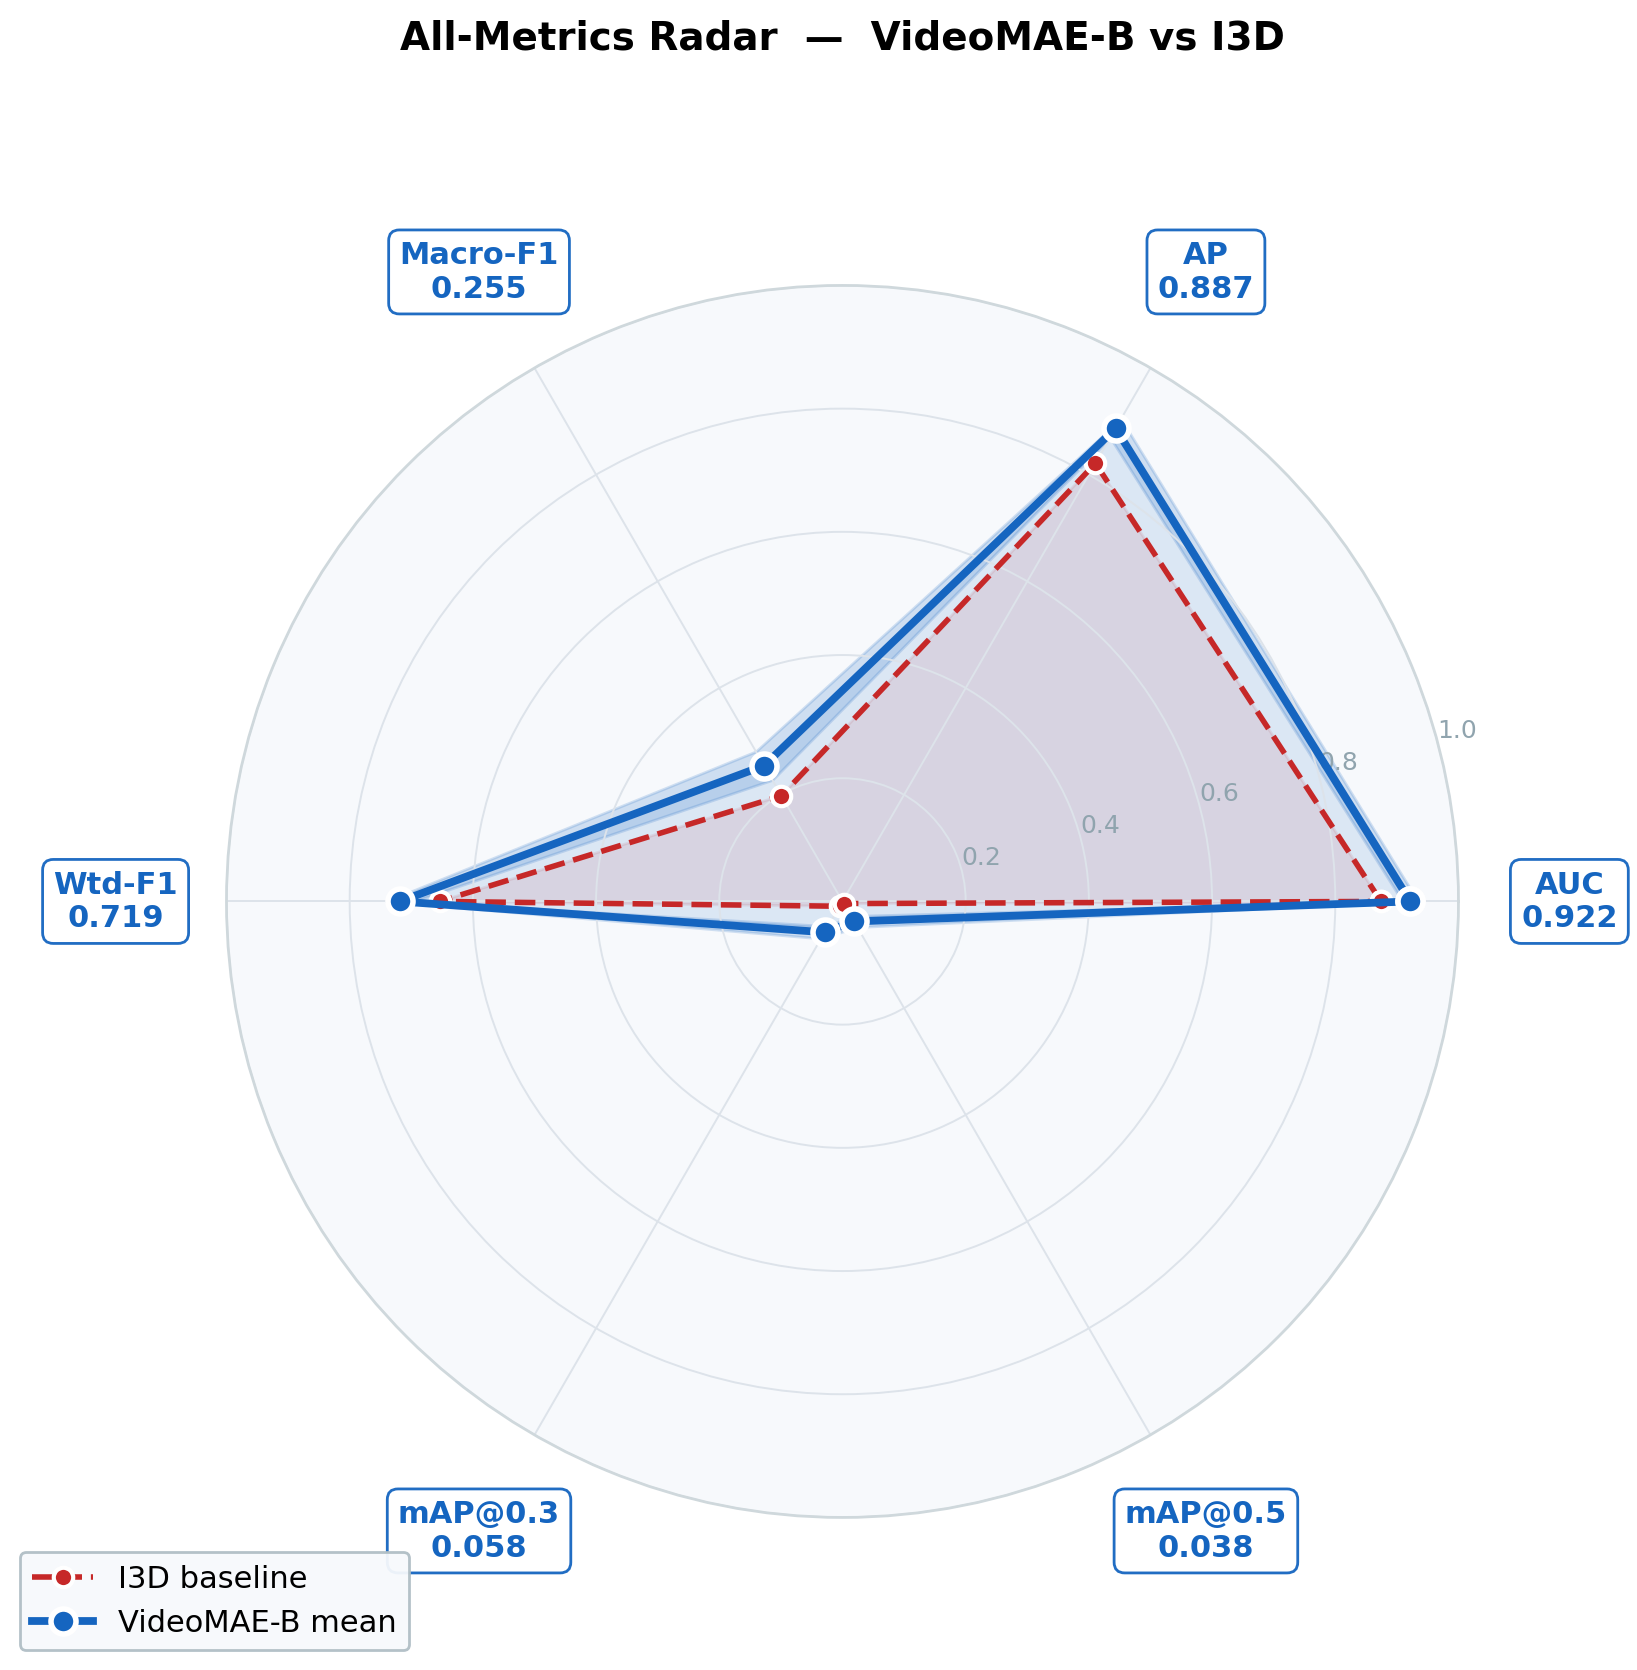
\includegraphics[width=0.88\linewidth]{figures/fig6_radar_overview.png}
  \caption{All-metrics radar---VideoMAE-B (blue, 3-seed mean) vs.\
           I3D baseline (red dashed). VideoMAE-B dominates every axis.}
  \label{fig:radar}
\end{figure}

\subsection{Discussion}
\label{sec:discuss}

\paragraph{Comparison caveat.}
Published SOTA rows in Table~\ref{tab:main} use frame-level AUC evaluated
on all 13 anomaly categories of UCF-Crime, while our rows use the 6-category
violence subset with video-level AUC.
These evaluations are \emph{not} directly comparable; we include published
numbers only to situate our work in the broader landscape.
Within our controlled I3D-vs-VideoMAE-B comparison, the backbone swap
yields $+$4.8\,pp AUC and ${\times}6.4$ mAP@0.3—a strong signal
regardless of evaluation differences.

\paragraph{Why localization improves most.}
VideoMAE's reconstruction pre-training forces the model to reason about
spatiotemporal continuity across masked patches, producing features that
encode temporal transitions more precisely than I3D's optical-flow stream.
These richer temporal representations may contribute to sharper event boundary
predictions, which would explain the disproportionate mAP gain at strict IoU
thresholds—though a dedicated boundary-head ablation is needed to isolate this
effect conclusively.

\paragraph{Cross-dataset transfer interpretation.}
XD-Violence binary transfer (ratio 0.901) confirms that VideoMAE-B violence
representations generalise well across camera domains when the anomaly
semantics overlap.
RWF-2000's strong AUC (0.862) but weak fight recall (0.14) points to a
calibration gap: the decision threshold is tightly tuned to UCF-Crime's
surveillance footage and penalises RWF's shorter, close-up clips.
ShanghaiTech's negative result (AUC 0.371) is expected by design—
non-violence anomalies are out-of-distribution for a violence-trained model.

\paragraph{Overall performance context.}
The binary detection results are strong in absolute terms: AUC\,92.2\% and
AP\,88.7\% are competitive with fully-supervised approaches on comparable
subsets, and the localization gains (${\times}6.4$--${\times}21.7$ mAP) are
substantial for a weakly-supervised system.
The one area where absolute performance is limited is Macro-F1 (0.255), but
this is a known artifact of severe class imbalance and scarce test samples for
rare categories (e.g., only 2 Abuse test videos), not a failure of the
VideoMAE-B representation itself.

\paragraph{Failure cases.}
The Fighting class collapse and the gap between Macro-F1 (0.255) and
Weighted-F1 (0.719) reveal that rare categories remain challenging.
Fighting shares motion statistics with normal crowded scenes, and 16-frame
context appears insufficient to capture the build-up dynamics that distinguish
a fight from ordinary movement; longer context windows or hierarchical
aggregation are natural remedies.
The RWF conservative recall further suggests calibration-aware thresholding
as a priority for future work.


%% ============================================================
\section{Conclusion}
\label{sec:conclude}
%% ============================================================

We demonstrated that replacing frozen I3D features with frozen VideoMAE-B
features in a weakly-supervised RTFM + TRN + Boundary Head pipeline yields
consistent, large improvements in violence detection and temporal localization
on the UCF-Crime violence subset ($+$4.8\,pp AUC, ${\times}6.4$ mAP@0.3).
Zero-shot transfer to XD-Violence remains strong for binary ranking
(AUC\,0.836, transfer ratio 0.901), with partial class-level transfer for
explosion and fighting.
RWF-2000 fight validation confirms useful anomaly ranking (AUC\,0.862) but
reveals conservative threshold behaviour under domain shift.
ShanghaiTech robustness is negative (AUC\,0.371), confirming that
violence-trained representations do not generalise to non-violence anomaly
semantics without retraining.
A lightweight training recipe—inverse-frequency class weights,
confidence-thresholded pseudo-labels, and cosine annealing LR—further
stabilises UCF-Crime results across seeds.

\paragraph{Limitations and future work.}
Macro-F1 remains low (25.5\%), driven primarily by the Fighting class
collapse under 16-frame segmentation.
Future directions include: (i)~calibration-aware thresholding to improve
external recall without increasing false positives, (ii)~longer-context
windows (32 or 64 frames) for fight-build-up capture,
(iii)~VideoMAE-Large backbone for richer representations, and
(iv)~domain adaptation for non-violence anomaly benchmarks such as
ShanghaiTech.


%% ============================================================
%% Author Contributions
%% ============================================================
\section*{Author Contributions}

\textbf{Srinivasa Sai Chava} conceived and led the entire project.
He designed and implemented the full pipeline from scratch: UCF-Crime violence-subset data preparation and class-balanced splits; frozen I3D and VideoMAE-B feature extraction and caching; the RTFM-style weakly-supervised MIL scorer; the event-classification head with confidence-thresholded pseudo-label generation; the TRN temporal-refinement module; the boundary-confidence head and tIoU-based decode-time refinement; and the composite training objective with inverse-frequency class weighting and cosine-annealing LR scheduling.
He ran all UCF-Crime training experiments (multi-seed sweeps, ablations), zero-shot cross-dataset evaluations on XD-Violence, RWF-2000, and ShanghaiTech, and the full interpretability package (error taxonomy, temporal-attention analysis, t-SNE feature-space visualisation, and boundary-precision analysis).
He wrote this paper.

\textbf{Yuxiang Liu} contributed auxiliary analysis and evaluation tooling.
He added threshold calibration and false-alarm analysis utilities, multi-run binary-accuracy and ablation reporting scripts, local experiment shell scripts, and extended evaluation entry points for multi-category UCF testing.
He also extended the core boundary analysis, error taxonomy, evaluation, dataset, and training modules with additional logging and reporting hooks, added feature utility helpers, and authored the repository README and results-tracking document.

\textbf{Vishakha} --

\textbf{Shristhy} conducted exploratory data analysis on the ShanghaiTech and UCF-Crime datasets.

\textbf{Anagha} --

%% ============================================================
%% References
%% ============================================================
\bibliographystyle{acl_natbib}
\bibliography{references}

\end{document}
